\documentclass[11pt]{article}

% Use wide margins, but not quite so wide as fullpage.sty
\marginparwidth=0.5in
\oddsidemargin0.25in
\evensidemargin0.25in
\marginparsep0.25in
\topmargin 0.25in 
\textwidth 6in \textheight 8 in
% That's about enough definitions

\usepackage{natbib}
\usepackage{float}
% multirow allows you to combine rows in columns
\usepackage{multirow}
% tabularx allows manual tweaking of column width
\usepackage{tabularx}
% longtable does better format for tables that span pages
\usepackage{longtable}
\usepackage{graphicx}
\graphicspath{{images/}}
\usepackage[section]{placeins}
\usepackage{booktabs}
\usepackage{caption}
\usepackage{listings} % for R code snippets
\usepackage[toc,page]{appendix}

\begin{document}
\author{Ryan Watkins}
\title{Data Mining: Major Coursework}
\maketitle
\pagebreak
\tableofcontents
\pagebreak

\section{Task 1 \- Data Exploration and Clustering}
Using the wine dataset, we explore clustering and PCA technique. PCA reduces the dimensionality of the data and organizes the data into principle components of original dimension size. The first PCA component has the highest variance, the second PCA component has the second highest variance and so on. It's usage is largely exploratory but can also be used for predictive modelling. It's usage can be thought of to show the structure of the variance within the data~\cite{dunteman1989principal}. Figure~\ref{fig:pca_un} shows PCA on the wine dataset unnormalised.

For clustering, K-means clustering is utilized. K-means clustering technique organizes points into groups using euclidian distance from centroids and a preset amount of centroids, the \textit{K}. Initial setup of the centroids is a research topic that has been widely explored~\cite{pelleg2000x},~\cite{arai2007hierarchical}. These centroids are somehow determined and then iteratively for each observation the nearest centroid is found by computing the distance between the observation and centroid for every centroid. After the observations are assigned a centroid, the centroids are recomputed by taking the average of the observations that now fall within the centroid. When there is no change in an iteration, convergence is reached. 

\begin{subsection}{Task1.1: Unnormalised PCA and K-means Clustering}
\begin{figure}[H]
    \centering
    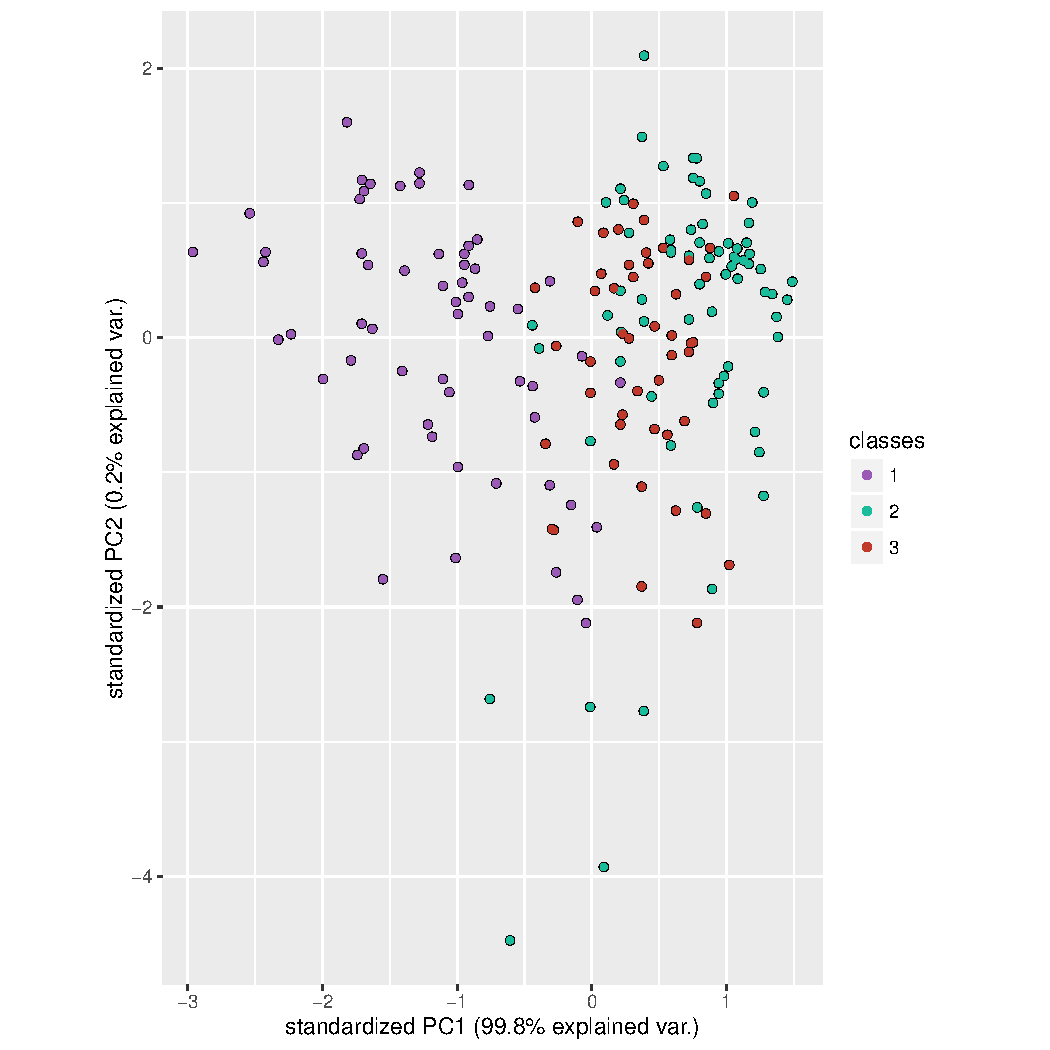
\includegraphics[width=0.9\textwidth]{p1_un}
    \caption{\textit{Plot 1.} PCA on Wine dataset unnormalised}
    \label{fig:pca_un}
\end{figure}

Performing clustering within \textit{R} can be done with the \textit{kmeans} function call from the library \textit{clustering}. Thus, clustering is performed with:

\begin{figure}[H]
\centering
\begin{lstlisting}[basicstyle=\ttfamily][language=R]
rm <- kmeans(wined[,2:14], 3)
autoplot(cd_k_unnorm, data=scale(wined[,2:14]))
\end{lstlisting}
\caption{R code which performs K-Means clustering on unnormalised wine dataset}
\label{fig:kmeans_r_code}
\end{figure}

\begin{figure}[H]
    \centering
    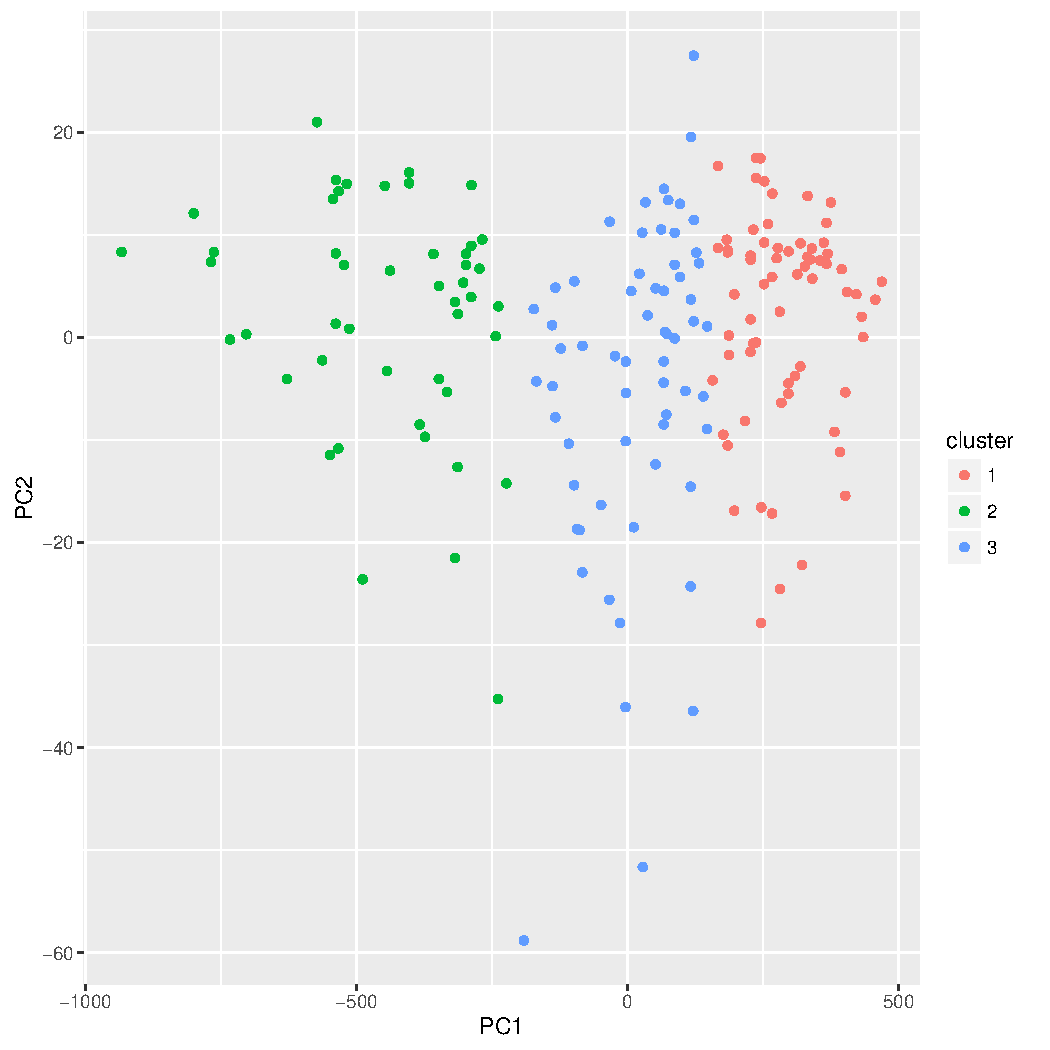
\includegraphics[width=1.0\textwidth]{p2_un}
    \caption{\textit{Plot 2.} K-means clustering on Wine dataset without normalisation with cluster amount set to three}
\end{figure}

One can visualize each cluster and begin to look closely at the class distributions within the clusters. This can be used to explore the data more. Figures~\ref{fig:p3a_un},~\ref{fig:p3b_un},~\ref{fig:p3c_un} demonstrates the class breakdown within each of the three clusters.
\begin{figure}[H]
    \centering
    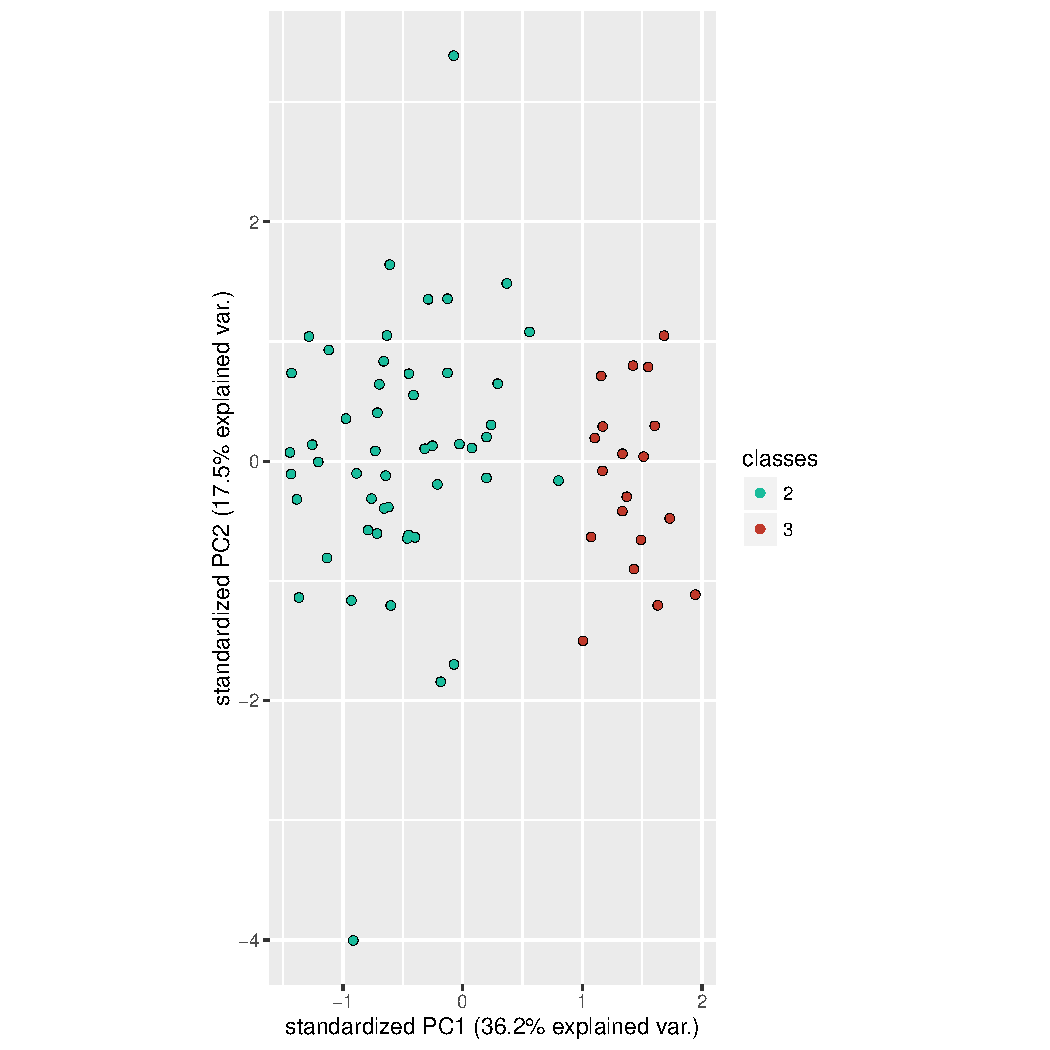
\includegraphics[width=1.0\textwidth]{p3a_un}
    \caption{\textit{Plot 3a.} 2D plot with class labelling for cluster one. The plot captures close to even proportion of class two and class three observations.}
    \label{fig:p3a_un}
\end{figure}

\begin{figure}[H]
    \centering
    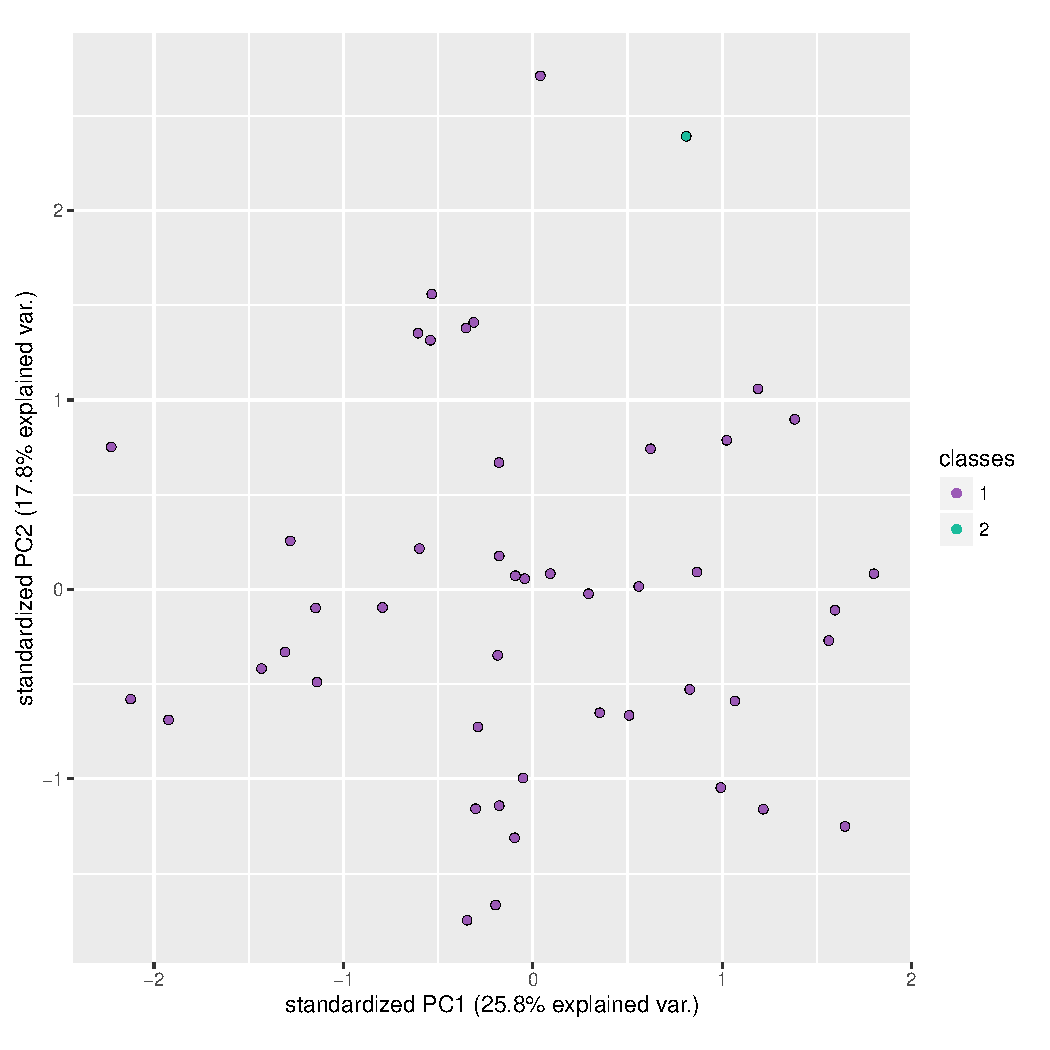
\includegraphics[width=1.0\textwidth]{p3b_un}
    \caption{\textit{Plot 3b.} 2D plot with class labelling for cluster two. Heavy observation of class one. One data point from class two.}
    \label{fig:p3b_un}
\end{figure}

\begin{figure}[H]
    \centering
    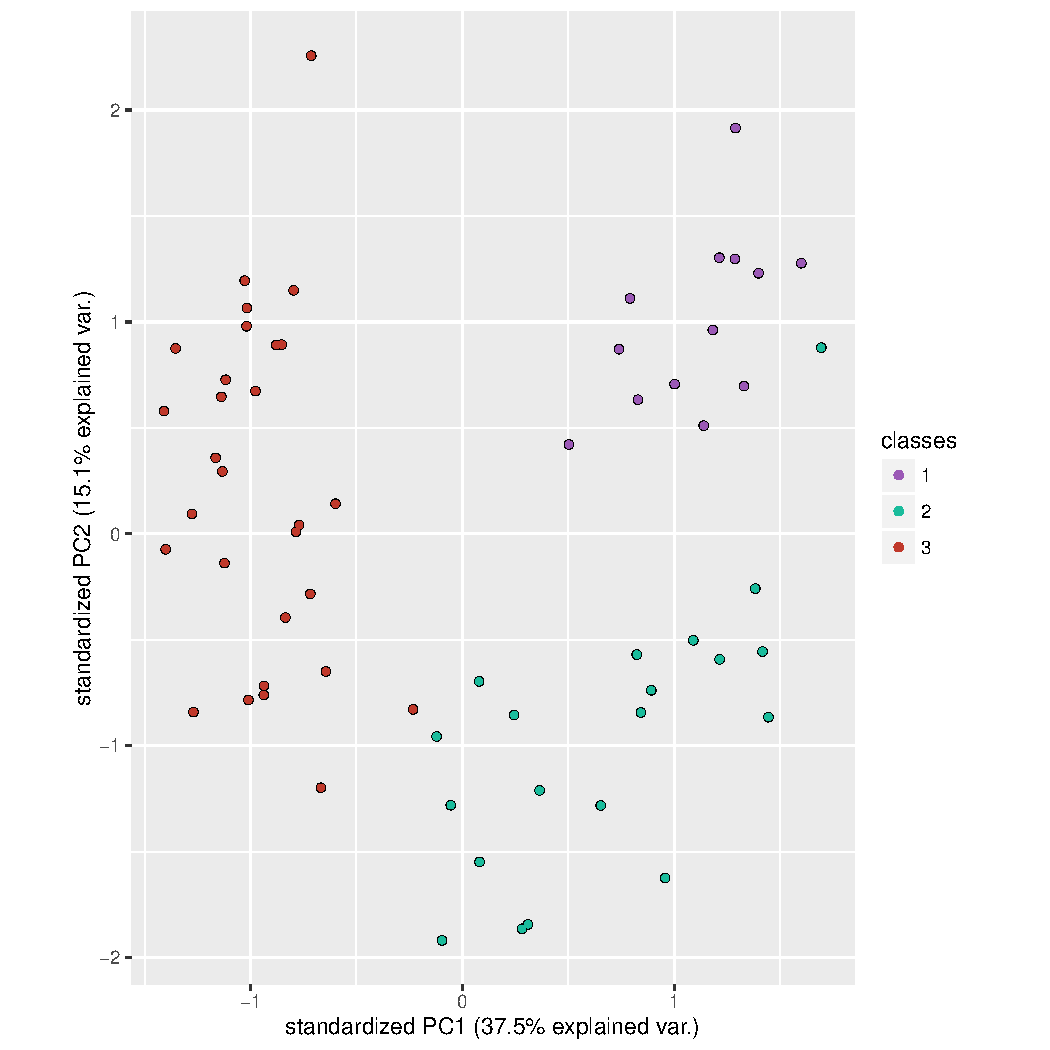
\includegraphics[width=1.0\textwidth]{p3c_un}
    \caption{\textit{Plot 3c.} 2D plot with class labelling for cluster three. Captures almost even distribution of all three classes.}
    \label{fig:p3c_un}
\end{figure}
\end{subsection}

\pagebreak\FloatBarrier\begin{subsection}{Task1.1: Cluster Validity}
    The package \textit{clValid}\cite{brock2011clvalid} is utilised from the CRAN repository to analyse and validify the clustering. \textit{clValid} contains three internal validity measures: Connectivity, Silhouette Width and Dunn Index. It can be used to compare multiple clustering methods also to determine which clustering method is best for the data.

    Connectivity indicates the degree of connectedness of the clusters, determined by k-nearest neighbours. It is a function that should be minimized~\cite{brock2011clvalid}.
    
    Silhouette Width is the average of the degree of confidence in the clustering assignment of a particular observation. It is a function that should be maximised in the range[-1,1]~\cite{brock2011clvalid}.
    
    The Dunn Index is the ratio of the smallest distance between observations not in the same cluster to the largest intra-cluster distance. Dunn Index should be maximised and has values between zero and infinity~\cite{brock2011clvalid}.
    
Below, Table 1 shows the validity results for the unnormalised wine dataset. The R code which implements the clustering validity is shown in Figure~\ref{fig:clustering_valid_r}

    \begin{figure}[H]
	\begin{lstlisting}[basicstyle=\ttfamily][language=R]
	# Attempt to perform cluster validation
	intern_unnorm <- clValid(wined[,2:14], 3, clMethods=c(
	  "clara", "kmeans", "hierarchical"), validation="internal")
	summary(intern_unnorm)
	\end{lstlisting}
	\caption{R code using \textit{clValid} for clustering validity on wine dataset. Compares Clara, K-Means and Hierarchical clustering.}
	\label{fig:clustering_valid_r}
    \end{figure}

 \begin{center}   
     \begin{tabular}{@{}llr@{}}
	\toprule[1.5pt]
	Measure & Value \\
	\toprule[1.5pt]
	Connectivity & 10.0151 \\ \midrule
	Dunn & 0.0193 \\ \midrule
	Silhouette & 0.5533 \\
	\bottomrule[1.25pt]
    \end{tabular}
 \captionof{table}{Internal clustering validity results for unnormalised wine dataset}

\end{center}
\end{subsection}

\pagebreak

\FloatBarrier\begin{subsection}{Task1.2: Normalised PCA and Clustering}
    PCA on the normalised wine dataset splits points into groups almost entirely by class which shows that clustering will be an easy task. Normalisation and PCA is performed as detailed in Figure~\ref{fig:norm_pca_r}. The \textit{scale} argument normalises the data. Figure~\ref{fig:norm_pca} shows the application of PCA on the wine normalised dataset.
    \begin{figure}[H]
	\centering
        \begin{lstlisting}[basicstyle=\ttfamily][language=R]
		df.pca <- prcomp(df[,2:14], scale. = TRUE)  
	\end{lstlisting}
	\caption{R code which normalises the wine dataset and applies PCA}
	\label{fig:norm_pca_r}
    \end{figure}


\begin{figure}[H]
    \centering
    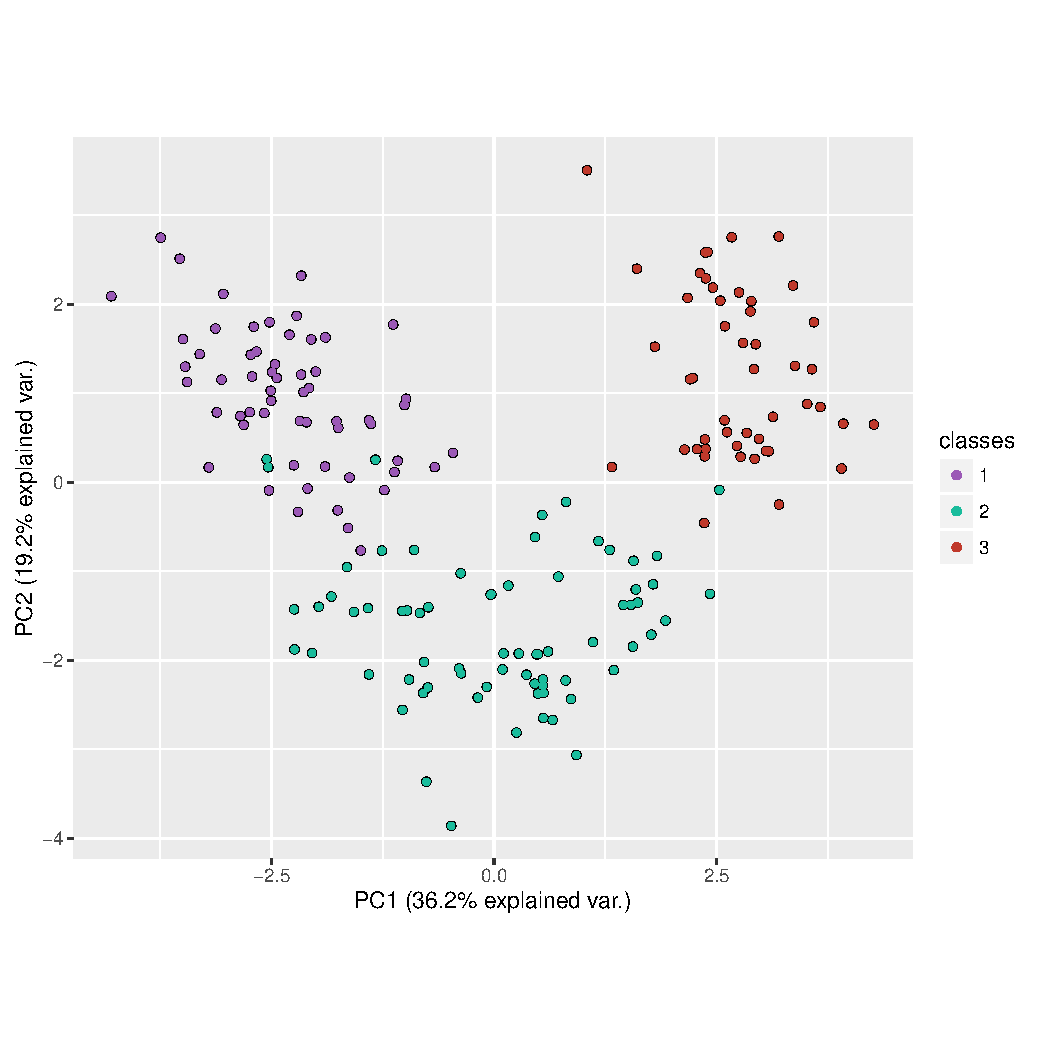
\includegraphics[width=1.0\textwidth]{p1_n}
    \caption{\textit{Plot 1. Normalised.} PCA on Wine dataset after normalisation}
    \label{fig:norm_pca}
\end{figure} \pagebreak


The K-means clustering technique on the normalised wine dataset derives well defined clusters. The clusters are formed in a different shape from the unnormalised dataset, instead there exists a `U shape'. Again, the R code calls \textit{kmeans} function and passes in the normalised data instead this time. Figure~\ref{fig:kmeans_norm} demonstrates K-Means on the normalised wine dataset. Figures~\ref{fig:p3a_n},~\ref{fig:p3b_n} and~\ref{fig:p3c_n} demonstrate the class breakdown in each of the three clusters.
\begin{figure}[H]
    \centering
    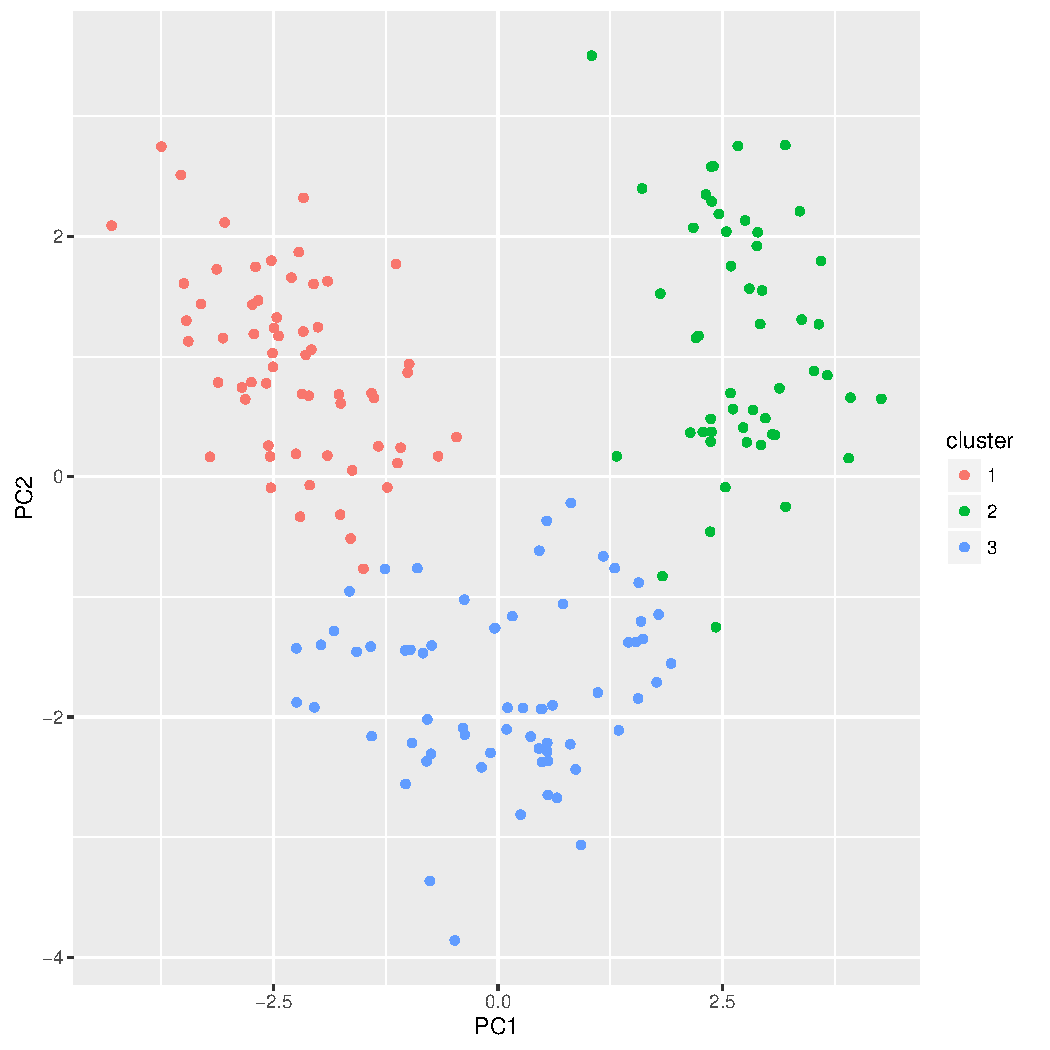
\includegraphics[width=1.0\textwidth]{p2_n}
    \caption{\textit{Plot 2. Normalised.} K-means clustering on Wine dataset with normalisation}
    \label{fig:kmeans_norm}
\end{figure}
\pagebreak Cluster one contains the vast majority of class one and a few observations from class two. In comparison to cluster one for the unnormalised wine dataset, there exists strong classification towards class one where-as cluster one in the unnormalised dataset had zero points from class one and no definitive labelling towards one class.
\begin{figure}[H]
    \centering
    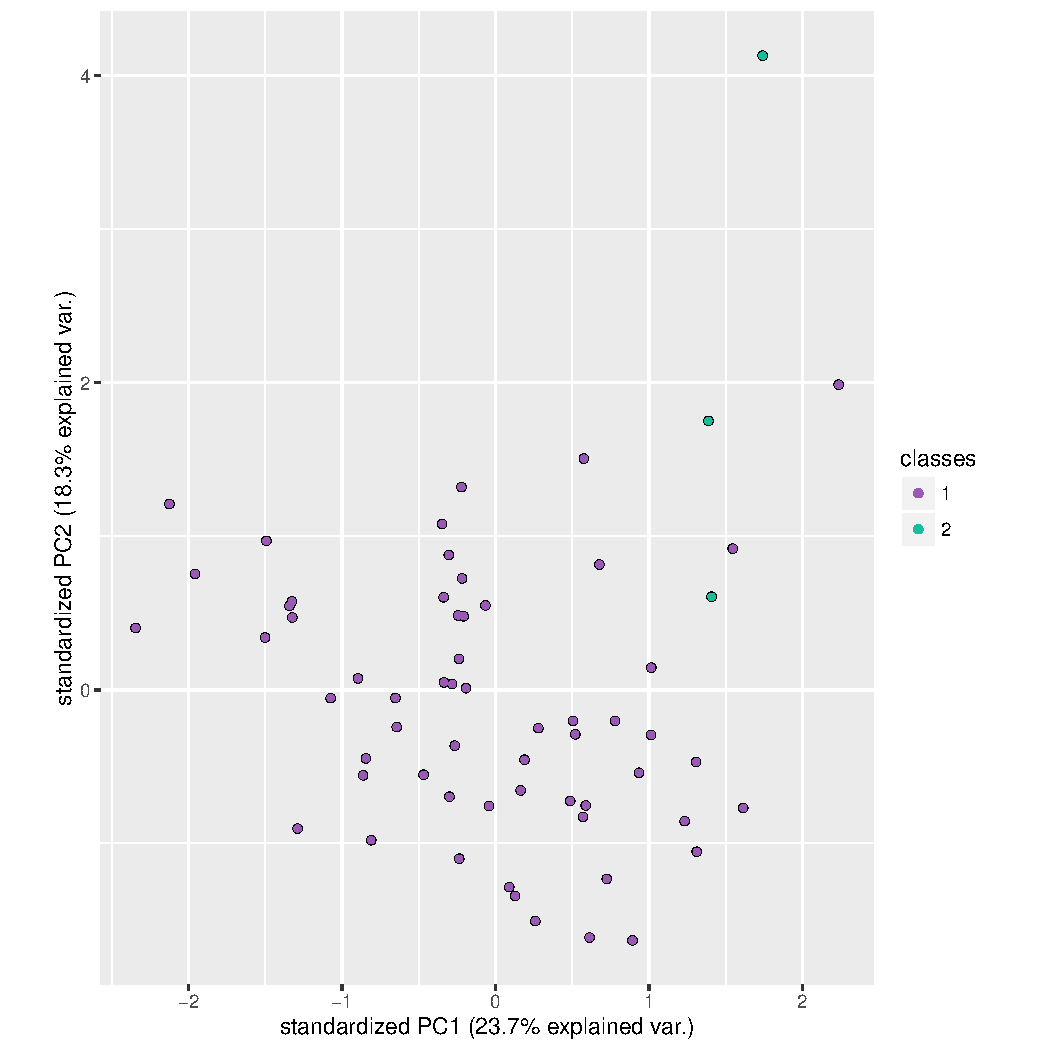
\includegraphics[width=1.0\textwidth]{p3a_n}
    \caption{\textit{Plot 3a. Normalised.} 2D plot with class labelling for cluster one after normalisation.}
    \label{fig:p3a_n}
\end{figure}
\pagebreak Cluster two contains strong classification towards class three.
\begin{figure}[H]
    \centering
    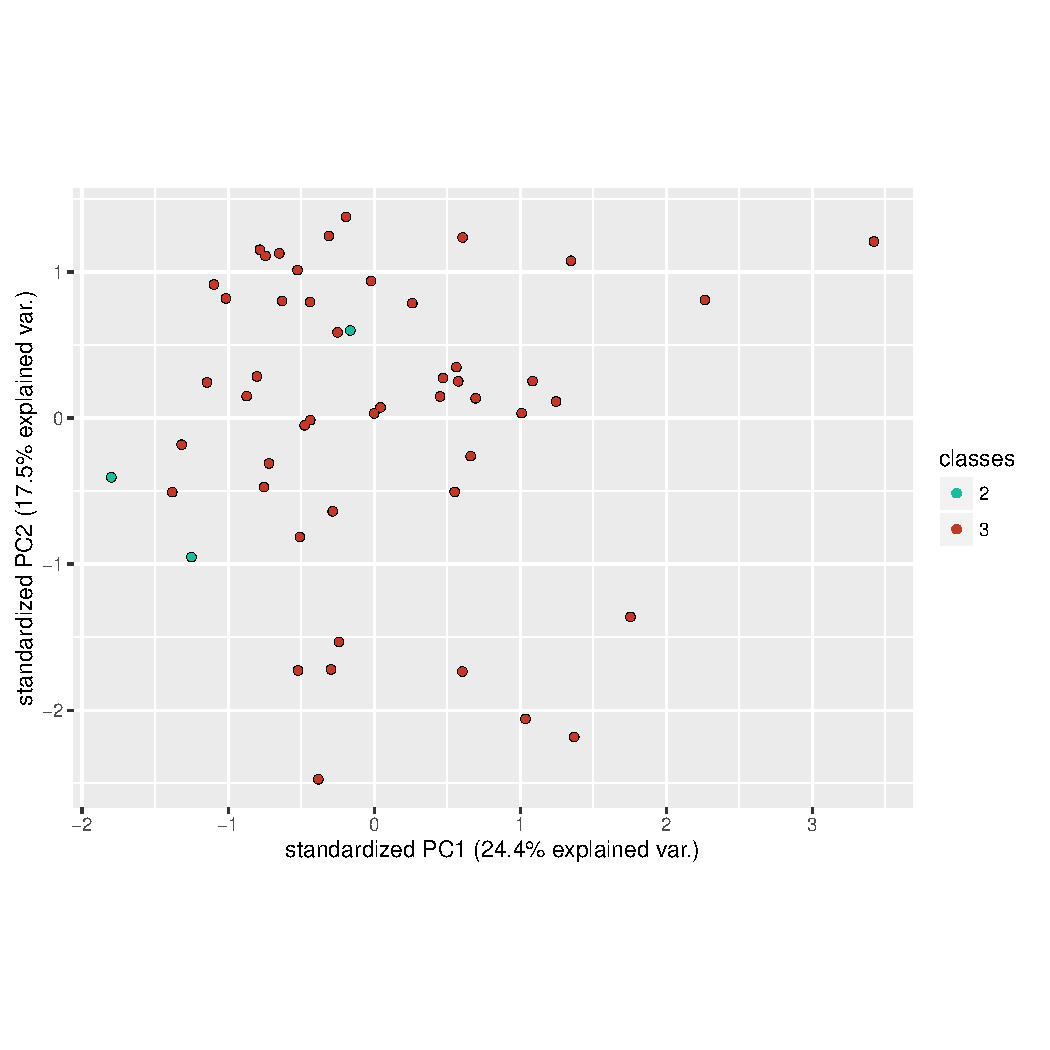
\includegraphics[width=1.0\textwidth]{p3b_n}
    \caption{\textit{Plot 3b. Normalised.} 2D plot with class labelling for cluster two after normalisation.}
    \label{fig:p3b_n}
\end{figure}
\pagebreak Cluster three contains points formed from class two. Again, one can observe that normalisation derives clusters which preserve classes better. The unnormalised wine dataset had an even distribution of all three classes in cluster three.
\begin{figure}[H]
    \centering
    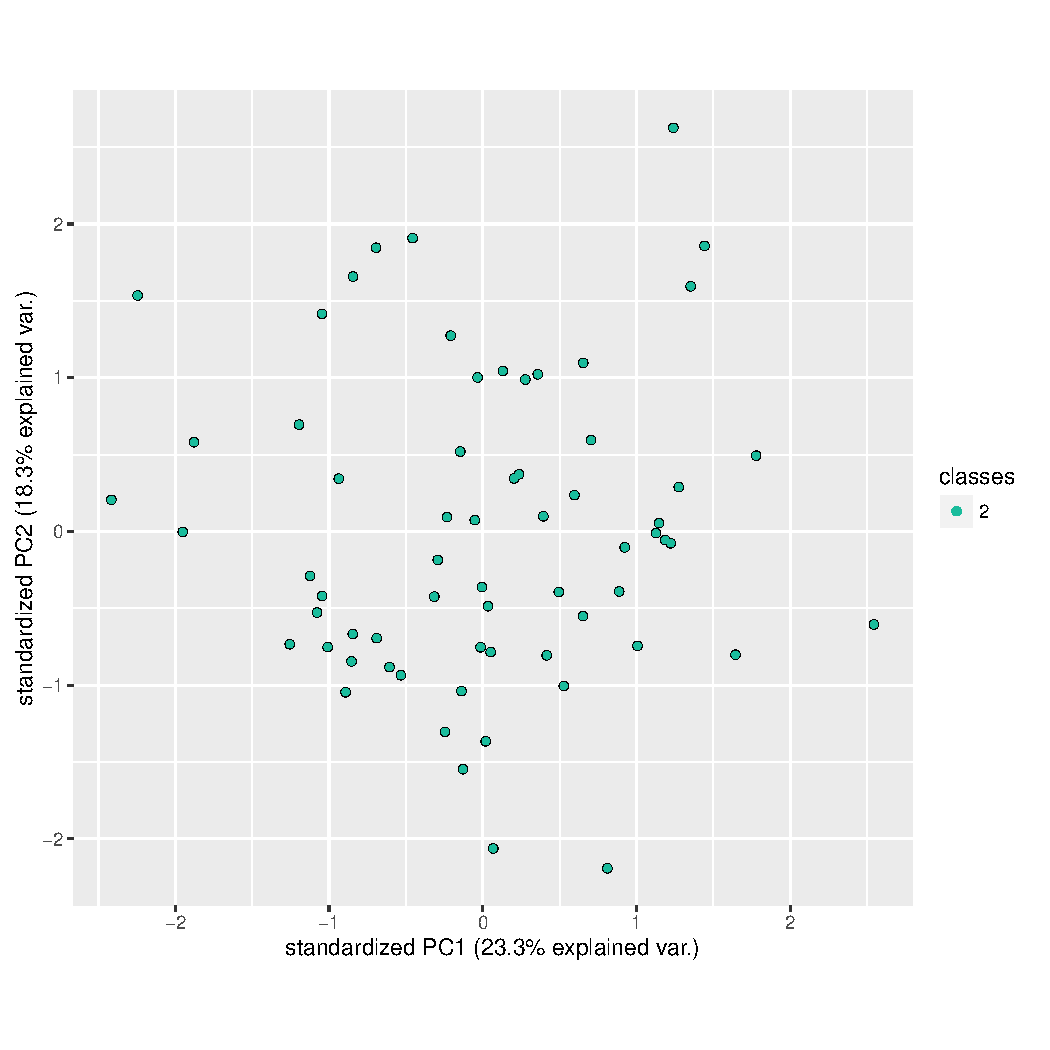
\includegraphics[width=1.0\textwidth]{p3c_n}
    \caption{\textit{Plot 3c. Normalised.} 2D plot with class labelling for cluster three after normalisation.}
    \label{fig:p3c_n}
\end{figure}
\end{subsection}

\pagebreak\begin{subsection}{Task1.2: Cluster Validity}
    The connectivity for the normalised dataset after performing k-means clustering technique performs worse than the unnormalised dataset. However, Dunn Index and Silhouette both perform better on the normalised dataset. Thus, the normalised dataset clusters better overall on these measures with K-means technique as two measures out of three are better for the normalised dataset. Below in Table 2 are the validity measure values for the normalised wine dataset. 
 \begin{center}   
 \begin{tabular}{@{}llr@{}}
	\toprule[1.5pt]
	Measure & Value \\
	\toprule[1.5pt]
	Connectivity & 28.0504 \\ \midrule
	Dunn & 0.2323 \\ \midrule
	Silhouette & 0.2849 \\
	\bottomrule[1.25pt]
    \end{tabular}
 \captionof{table}{Internal clustering validity results for normalised wine dataset}
\end{center}
\end{subsection}
\begin{subsection}{Conclusion}
    It is clear that normalisation for the wine dataset helps with classification and this is easy to see visually. Using a variety of clustering validity measures helps as you can take a majority vote on the \textit{winners} from the measures. This helps to verify further that the clustering method is better than the other. 
    
Utilizing PCA is good for visualizing high-dimensional data. PCA Analysis is critical within data mining as visualizing and exploring high dimensionality data is highly important during the pre-processing stage to see the variance in the data or more general attributes that \textit{describe} the data as a whole. 

A data scientist can begin to make important decisions in the pre-processing and data exploration stage which will derive a better result during classification or prediction in later stages. For instance, a data scientist may discover noise within the dataset upon applying PCA or other pre-processing techniques and begin to discard unimportant attributes also (feature selection).
\end{subsection}

\pagebreak\section{Task 2: Comparison of Classification Models}
KNN and Decision Trees are used to perform classification on the wine dataset. Ten-fold cross-validation is used to generate generalisation error and provide validity.

\subsection{Ten-fold cross-validation}
Ten-fold cross-validation is performed by holding out data across a dataset ten times, such that a 90\%/10\% split is obtained for train and test respectively until the entire dataset has been tested and trained. During each holdout, one performs classification and stores results for analysis after the iterative cycle of the ten folds has finished. Shuffling the data and picking data in the folds such that the class balance is preserved is important and utilized in ten-fold cross-validation techniques. There is a ten-fold cross-validation loop which makes folds and runs the process inside a for loop that iterates ten times. Ten-fold cross-validation has been studied in~\cite{kohavi1995study}. The implementation can be found inside \textit{dm\_2\_dt.R} and \textit{dm\_2\_knn.R}.

\subsection{Decision trees}
The package \textit{rpart} is used to form the tree using Breiman et al's Classification and Regression Trees (CART) method\cite{breiman1984classification}. The method minimizes the error in each leaf of the tree. No cost matrix or weighting is necessary in modelling as classes are well distributed. It's a good model for describing data. Other decision tree algorithms include ID3, C4.5 and C5.0. Figure~\ref{fig:t2_tree} demonstrates application of CART Decision Tree technique on the wine dataset. 
\begin{figure}[H]
    \centering
    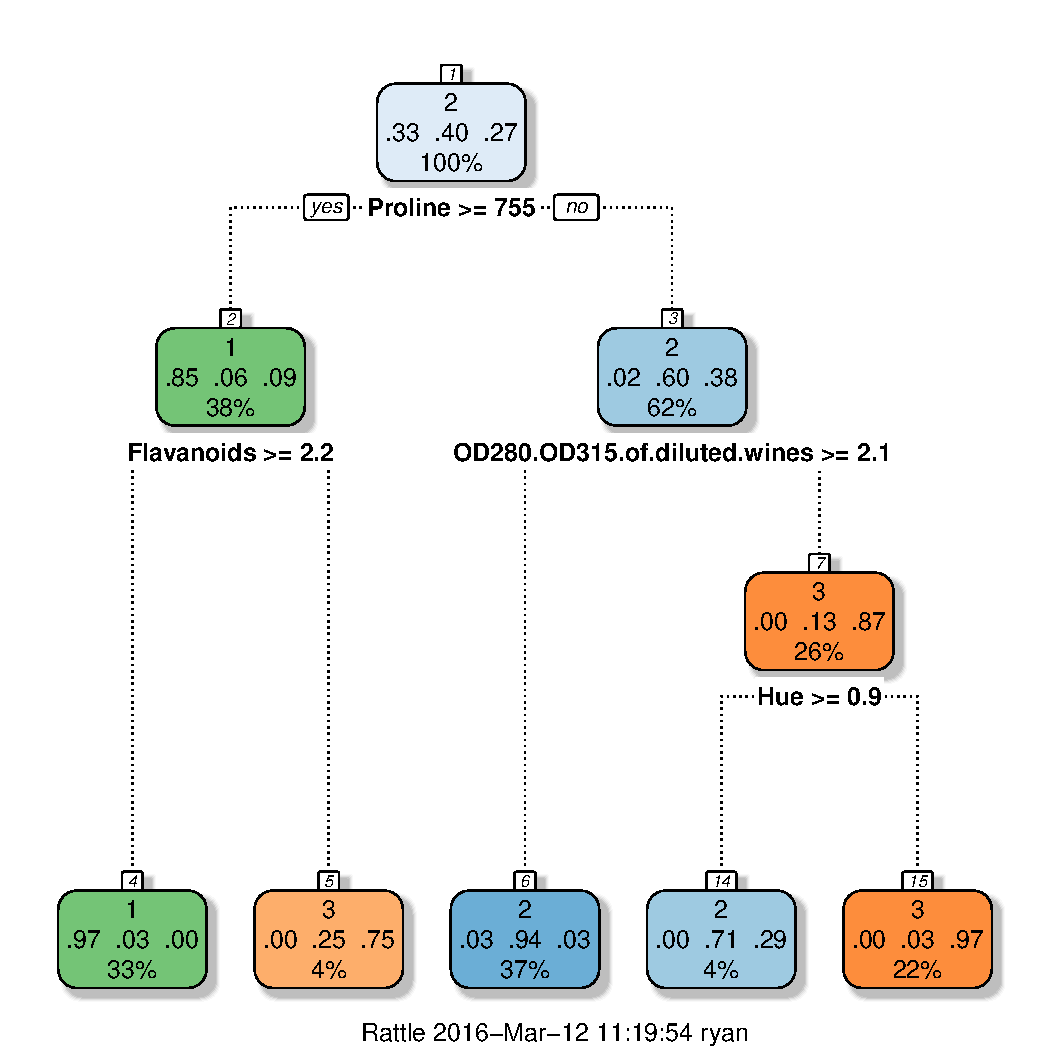
\includegraphics[width=0.7\textwidth]{t2_tree}
    \caption{Decision tree model using \textit{rpart} on wine dataset}
    \label{fig:t2_tree}
\end{figure}

\pagebreak Using \textit{plotcp}, possible cost-complexity prunings can be visualized and interpreted accordingly. \textit{plotcp} is used below on one fold. Figure~\ref{fig:t2_tree_prune} indicates that 0.017 is the best value to pick for pruning. Tree pruning has been studied in~\cite{cestnik1991estimating}. However, results show later that pruning was unnecessary as the \textit{rpart} function had already taken care of pruning.
\begin{figure}[H]
    \centering
    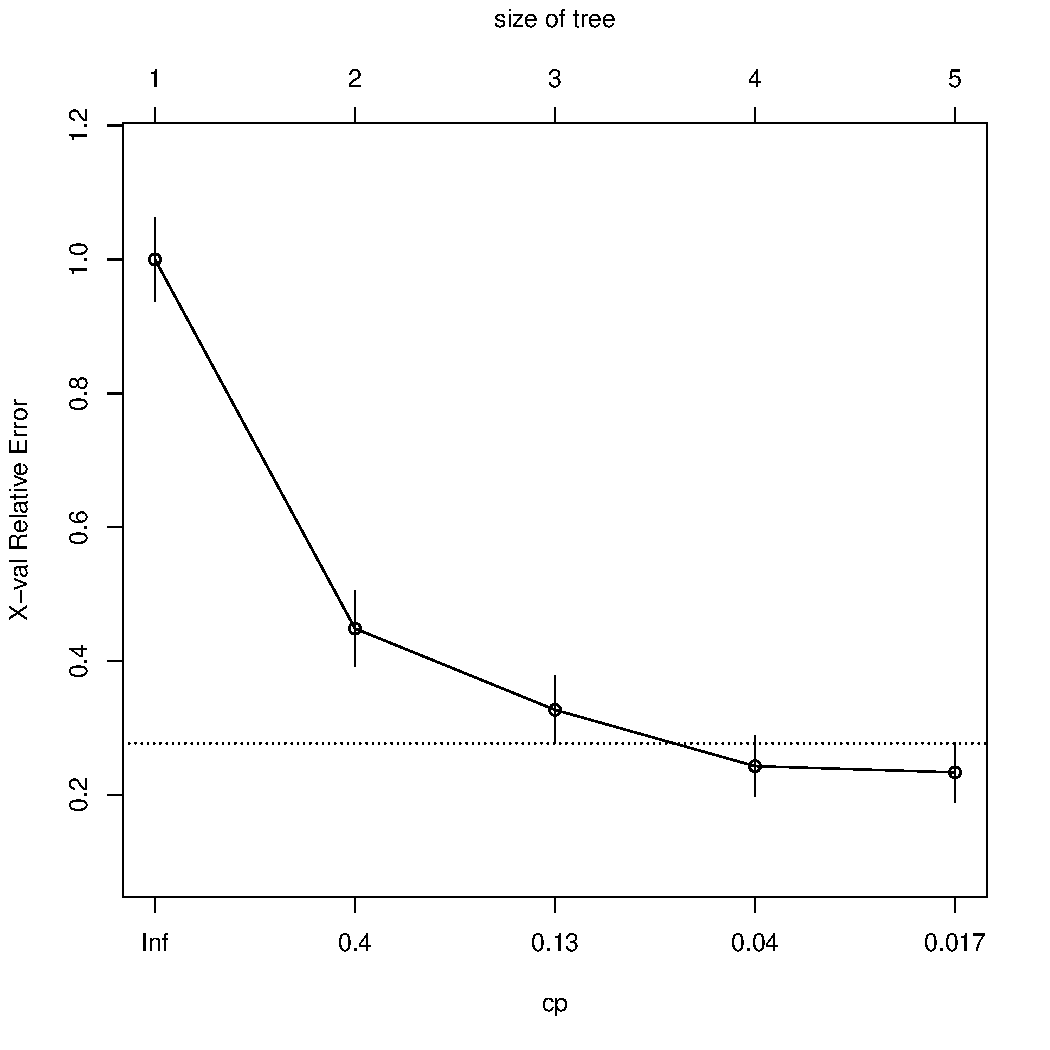
\includegraphics[width=1.0\textwidth]{t2_tree_prune}
    \caption{Tree pruning plot in R, useful for interpreting how to prune}
    \label{fig:t2_tree_prune}
\end{figure}

\pagebreak\subsection{KNN}
KNN is an algorithm that slowly and accurately classifies data. It classifies by taking a majority class vote on $K$ nearest neighbours. Getting K-selection correct is important and thus as a rule of thumb, $K=n^\frac{1}{2}$ is used. Using R's built-in \textit{knn} function, a generalisation error rate of 0.03954248 is derived. 

\subsection{Comparison Results}
A ROC curve would have been useful for analysing the classification methods, however they require binary classification. A workaround is the usage of Multi-class Area Under the Curve (AUC) as described by Hand and Till~\cite{hand2001simple}. The package \textit{pROC} provides multi-class AUC in R. 

Table~\ref{table:t2_class_comparisons} compares the two classification algorithms. The table demonstrates that KNN performs better classification on the dataset. Figure~\ref{fig:t2_tree} shows Decision Tree's descriptive power.

 \begin{center}   
 \begin{tabular}{@{}llr@{}}
	\toprule[1.5pt]
	Classifier & Measure & Value \\
	\toprule[1.5pt]
	KNN & Generalisation error & 0.03954248\\ \midrule
	KNN & Multi-level AUC & 0.979 \\ \midrule
        Decision Tree & Generalisation error & 0.0620915.\\ \midrule
	Decision Tree & Multi-level AUC & 0.9701 \\
	\bottomrule[1.25pt]
    \end{tabular}
 \captionof{table}{Comparison of Decision Trees and KNN on wine dataset}
 \label{table:t2_class_comparisons}
 \end{center}

 \subsection{Conclusion}
 Comparing classification methods is useful for data scientists as different classification methods work for different problems. It could be that classification accuracy is not the only metric that is important and instead there is a need to describe the data. In this case, decision trees would be picked as opposed to KNN technique. Likewise, performance constraints could also affect choice. KNN is known to be slow on massive datasets and instead perhaps a Neural Network may run faster or indeed regression or decision trees. There is no one-size fits all solution and it's always good to compare and constrast solutions before deciding on using a classification technique.

\pagebreak
\section{Task 3: The Search for God Particle: a Binary Classification Challenge}
A training dataset is provided such that there are 28 attributes and one class. The first 21 attributes comprise the low-level components measured as kinematic properties by particle detectors. The attributes thereafter comprise high level attributes which are made using a complex model as function of the low-level attributes (feature transformation). The task is to classify a dataset that only contains the 21 low-level attributes.

\subsection{Imbalanced Dataset Fixing}
A quick look at the dataset shows the distribution of classes as in Table~\ref{table:t3_class_dist}. The dataset is too imbalanced. An even distribution is needed before running ten-fold cross-validation. Figure~\ref{fig:t3_balance_r} shows R code that achieves a balancing of two classes. The class imbalance problem is studied in~\cite{japkowicz2002class}.

 \begin{center}   
 \begin{tabular}{@{}llr@{}}
	\toprule[1.5pt]
	Class & Amount\\
	\toprule[1.5pt]
	Background & 89999\\ \midrule
	Signal & 10000\\ 
	\bottomrule[1.25pt]
    \end{tabular}
 \captionof{table}{Class distribution in Hadron Collider training dataset}
 \label{table:t3_class_dist}
 \end{center}

 \begin{figure}[H]
\begin{center}
    \begin{lstlisting}[basicstyle=\ttfamily][language=R]
even.class.distribution <- function () {
  train100k <- train100k[sample (nrow (train100k)),] # Shuffle data

  classd <- train100k[which (train100k[,29]==0),]
  based <- train100k[which (train100k[,29]==1),]
 
  ind <- sample (1: (100000-nrow (based)), 10000)
  train100k.evenSplit <<- rbind (classd[ind,],based)
  train100k.evenSplit <<- train100k.evenSplit[sample 
                          (nrow (train100k.evenSplit)),] # Reshuffle
}
\end{lstlisting}
\end{center}
\caption{R code to split class distribution evenly}
\label{fig:t3_balance_r}
\end{figure}

\pagebreak
\subsection{Forming model for High Level Components}
An hypothesis is the seven high level components will help classification. Linear Regression is employed to estimate the high-level attributes using the \textit{lm} function in R. The model is made using the first twenty-one low-level attributes. Table~\ref{table:t3_model_res} shows the room mean squared errors (RMSE) for each of the 7 high-level components averaged across ten folds in ten-fold validation using the evenly split dataset formed from \textit{even.class.distribution()}.

 \begin{center}   
 \begin{tabular}{@{}llr@{}}
	\toprule[1.5pt]
	HL Attr. & Avg. RMSE\\
	\toprule[1.5pt]
	1 & 0.6497242\\ \midrule
	2 & 0.3587509\\ \midrule
	3 & 0.1530353 \\ \midrule
	4 & 0.3611804\\ \midrule
	5 & 0.4137971\\ \midrule 
	6 & 0.2930333\\ \midrule
	7 & 0.2559048\\ \midrule
	Total avg & 0.3550609\\
	\bottomrule[1.25pt]
    \end{tabular}
 \captionof{table}{Average errors after linear regression on the 7 high level attributes during 10-fold cross-validation}
 \label{table:t3_model_res}
 \end{center}

\subsection{Classification on train100k}
Classification models are built and evaluated on the original dataset using ten-fold cross-validation with datasets containing just low-level values, just regressed high-level attributes, scaled original data and also a combination of original low-level and regressed high-level attributes. The classification methods are logistic regression and neural networks. 

During the ten-fold cross-validation \textit{for} loop, each different dataset is formed and evaluated using both aforementioned techniques. To form the datasets, one must regress the high level attributes during each loops and replace the high level data within the training and test datasets. This is accomplished by the function \textit{get.high.levels}. The holdout data is reset after each iteration of the ten-fold cross-validation using a defined function \textit{reset.holdout.data}. The two functions \textit{logit.classification} and \textit{nn.classification} run the logistic regression and neural network classifcation respectively. 

\subsection{Results for classification on train100k}
A breakdown is shown in Table~\ref{table:t3_class_res}. All measure values are averaged across ten folds. ROC Curves are given in Figures~\ref{fig:t3_roc_low},~\ref{fig:t3_roc_reg_hl},~\ref{fig:t3_roc_scaled} and~\ref{fig:t3_roc_low_reg_hl}. Accuracy curves are shown in Figures~\ref{fig:t3_acc_low},~\ref{fig:t3_acc_reg_hl},~\ref{fig:t3_acc_scaled} and~\ref{fig:t3_acc_low_reg_hl}. A key statistic is that the best \textit{low.reg.hl} accuracy was 0.613. It's model is utilized later to predict the new dataset with missing components. The results infer which model will work best on the unknown data. It should be noted though that the scaled dataset is not feasible for application on the unknown data as the high level components are unknown in the unknown data.
% Results table
\begin{center}   
 \begin{tabular}{@{}lllllr@{}}
	\toprule[1.5pt]
	Classifier & Dataset & Accuracy & Precision & Recall & F-measure\\
	\toprule[1.5pt]
	Logistic Regression & low & 0.5619 & 0.5610363 & 0.5694674 & 1.708402 \\
	Logistic Regression & reg.hl & 0.5756 & 0.5795118 & 0.5516499 & 1.65495  \\
	Logistic Regression & scaled & 0.63415 & 0.6021862 & 0.7922165 & 2.376649 \\
	Logistic Regression & low.reg.hl & 0.5619 & 0.5610363 & 0.5694674 & 1.708402 \\
	Neural Network & low & 0.5961 & 0.598144 & 0.5858072 & 1.757421 \\
	Neural Network & reg.hl & 0.5984 & 0.5980422 & 0.6013244 & 1.803973 \\
	Neural Network & scaled & 0.6884 & 0.6890128 & 0.6878997 & 2.063699 \\
	Neural Network & low.reg.hl & 0.5977 & 0.5993678 & 0.5914822 & 1.774447 \\
	\bottomrule[1.25pt]
    \end{tabular}
    \captionof{table}{Classification results: four datasets, two classification methods and four measures}
    \label{table:t3_class_res}
 \end{center}

\begin{figure}[H]
  \centering
    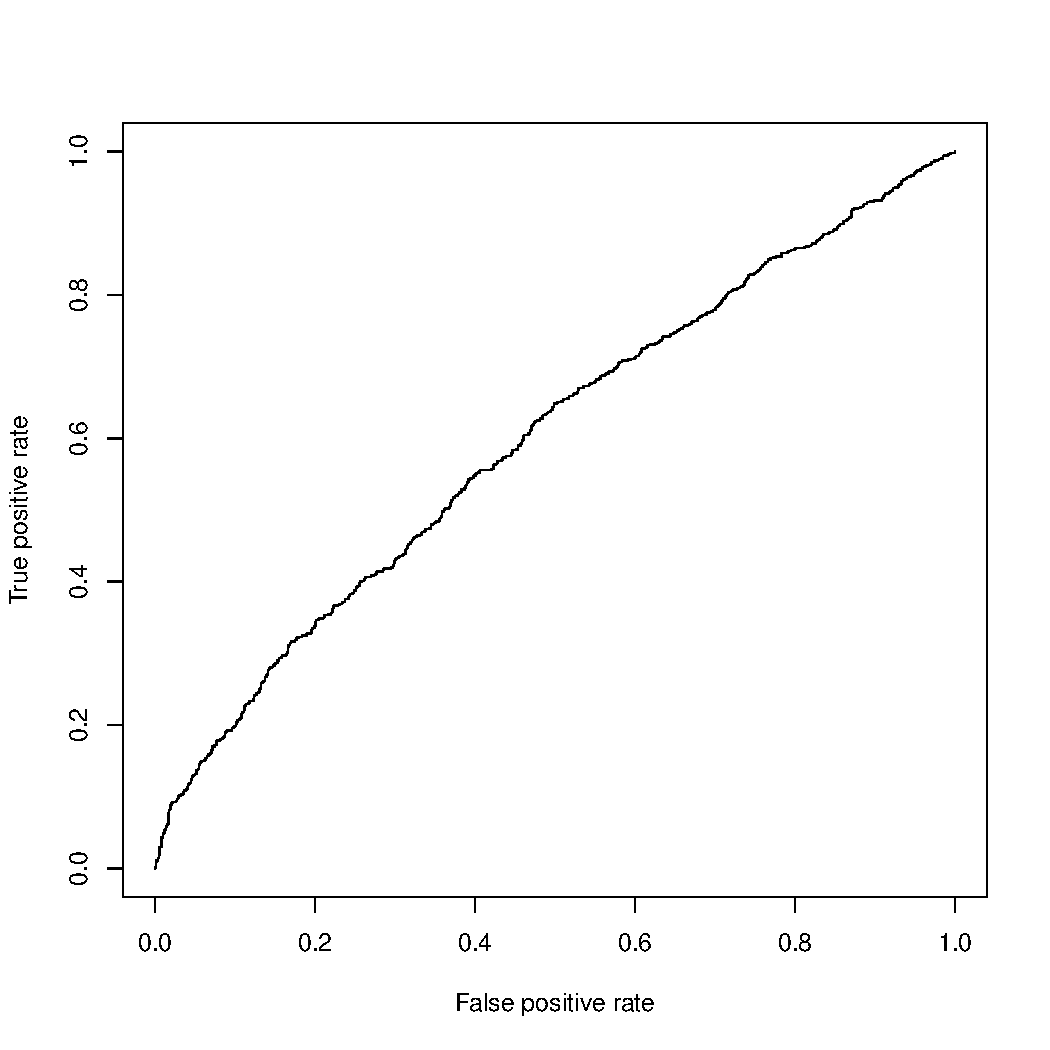
\includegraphics[width=0.9\textwidth]{t3/roc_low}
    \caption{ROC Curve on low-level attributes logistic regression model during last fold of ten-fold cross-validation}
    \label{fig:t3_roc_low}
\end{figure}

\begin{figure}[H]
  \centering
    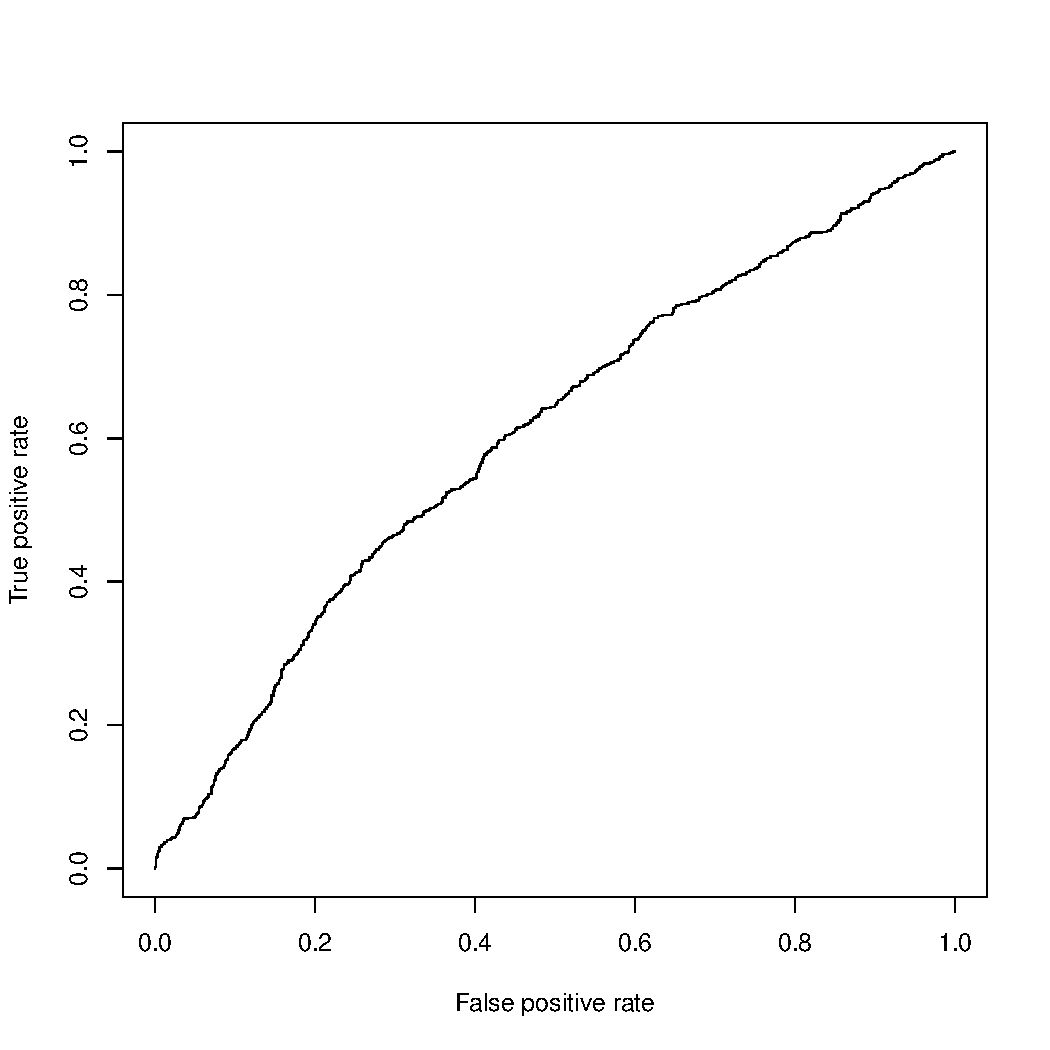
\includegraphics[width=0.9\textwidth]{t3/roc_reg_hl}
    \caption{ROC Curve on just high level regressed attributes logistic regression model during last fold of ten-fold cross-validation}
    \label{fig:t3_roc_reg_hl}
\end{figure}
\begin{figure}[H]
  \centering
    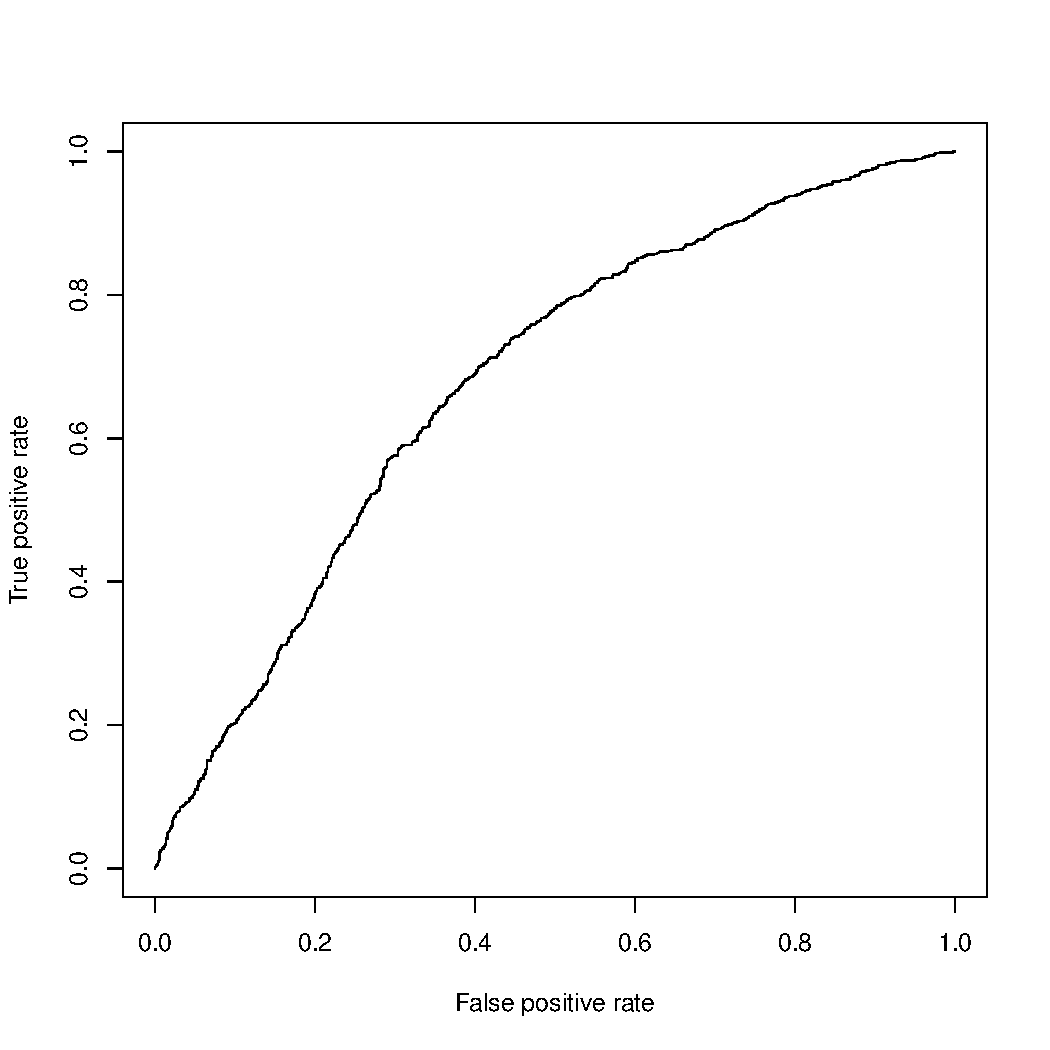
\includegraphics[width=0.9\textwidth]{t3/roc_scaled}
    \caption{ROC Curve on scaled dataset logistic regression model during last fold of ten-fold cross-validation}
    \label{fig:t3_roc_scaled}
\end{figure}

\begin{figure}[H]
  \centering
    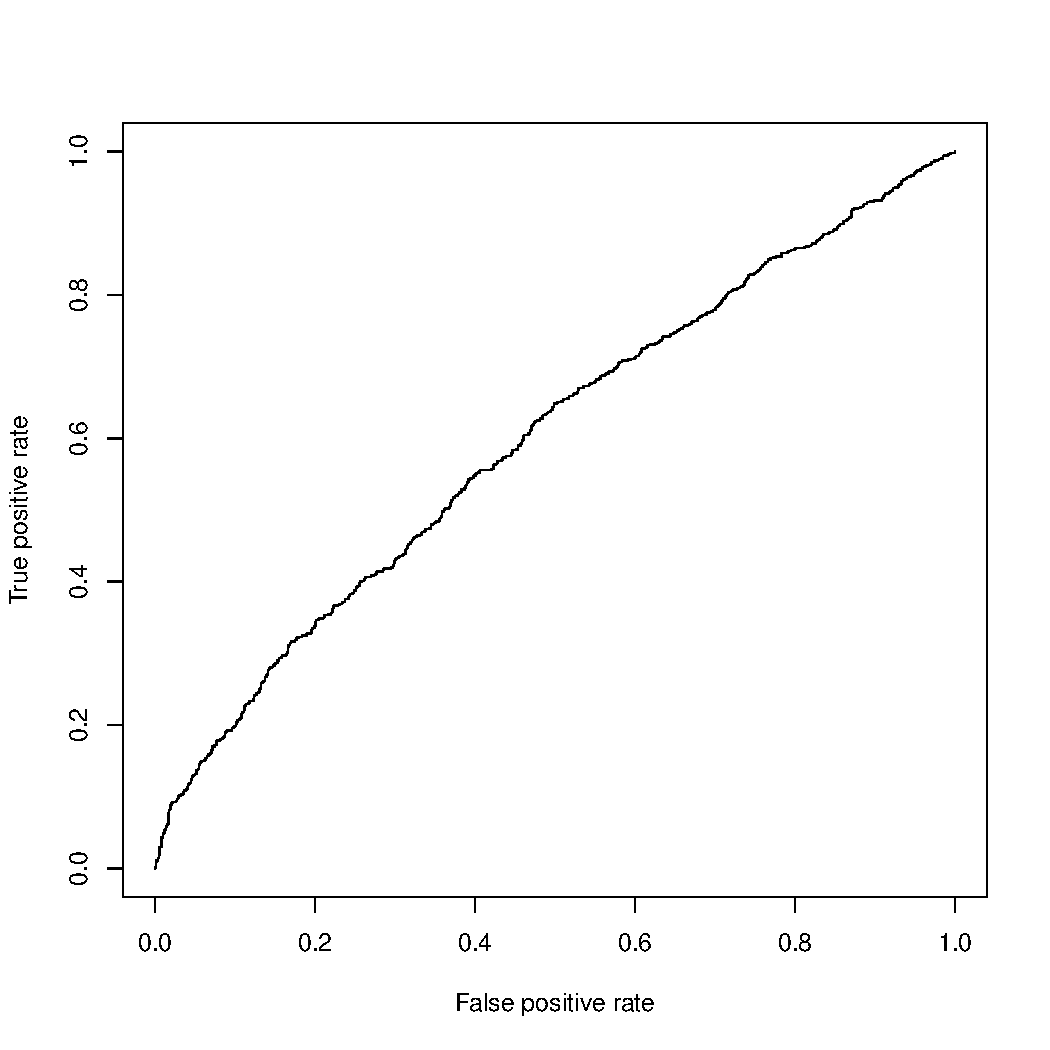
\includegraphics[width=0.9\textwidth]{t3/roc_low_reg_hl}
    \caption{ROC Curve on combination of low-level attributes and regressed high-level attributes logistic regression model during last fold of ten-fold cross-validation}
    \label{fig:t3_roc_low_reg_hl}
\end{figure}

\begin{figure}[H]
  \centering
    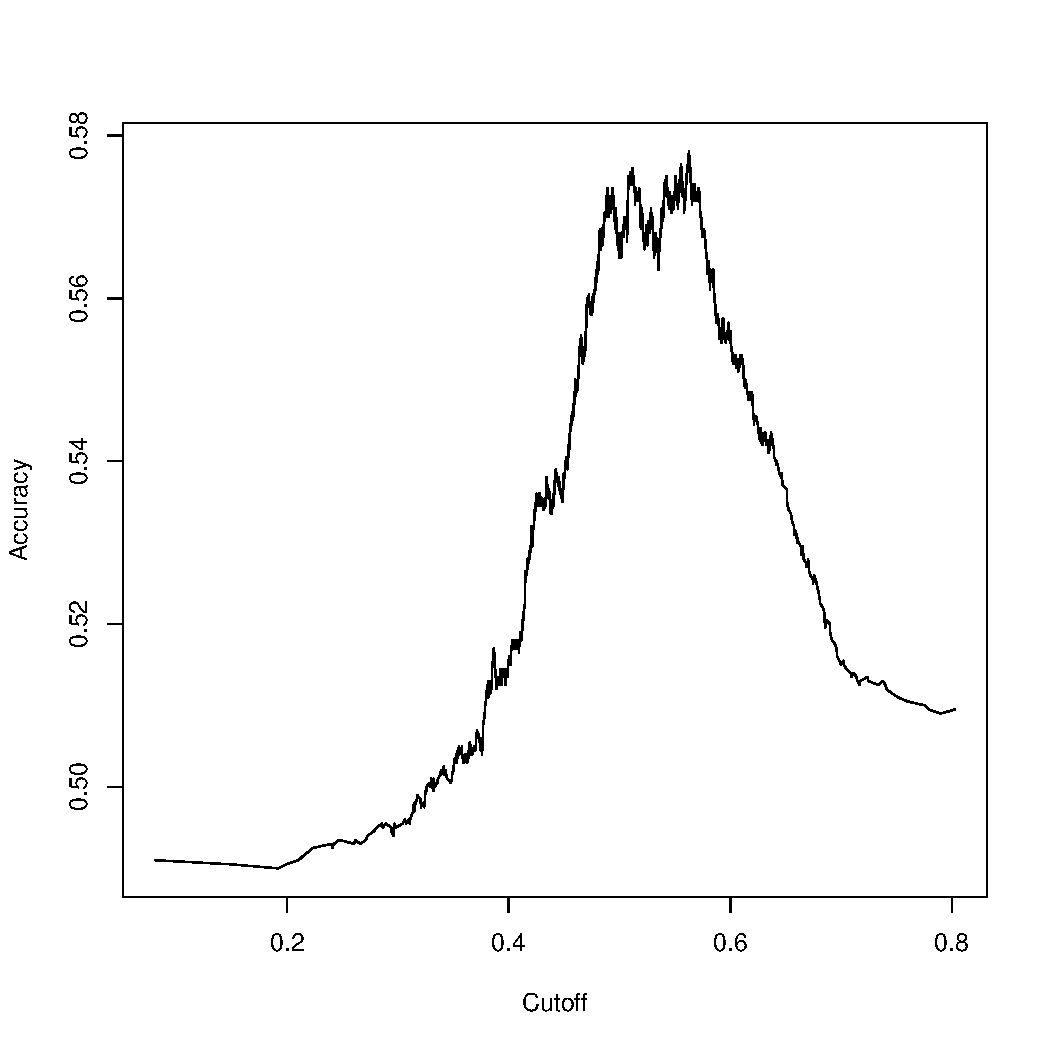
\includegraphics[width=0.9\textwidth]{t3/acc_low}
    \caption{Accuracy Curve on low-level attributes logistic regression model during last fold of ten-fold cross-validation}
    \label{fig:t3_acc_low}
\end{figure}

\begin{figure}[H]
  \centering
    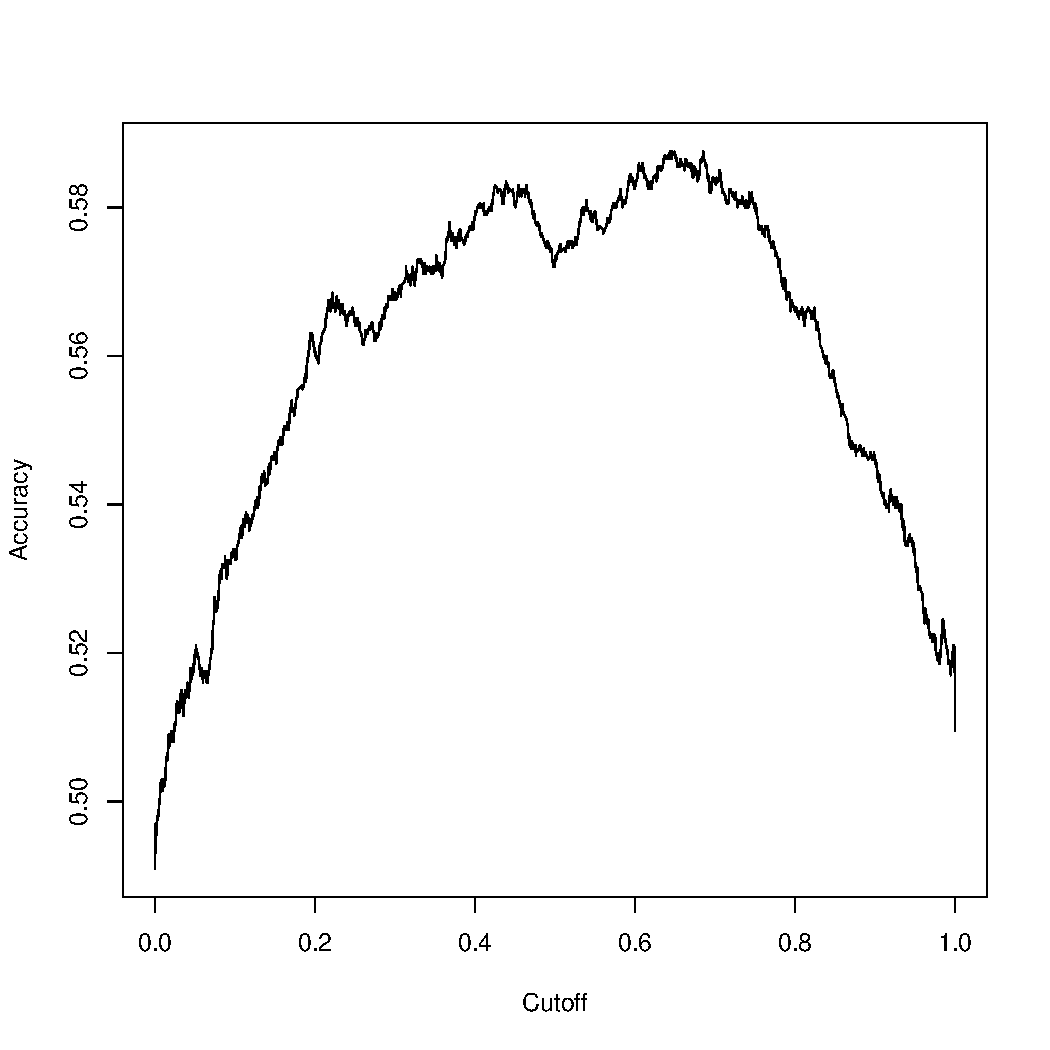
\includegraphics[width=0.9\textwidth]{t3/acc_reg_hl}
    \caption{Accuracy Curve on just high level regressed attributes logistic regression model during last fold of ten-fold cross-validation}
    \label{fig:t3_acc_reg_hl}
\end{figure}
\begin{figure}[H]
  \centering
    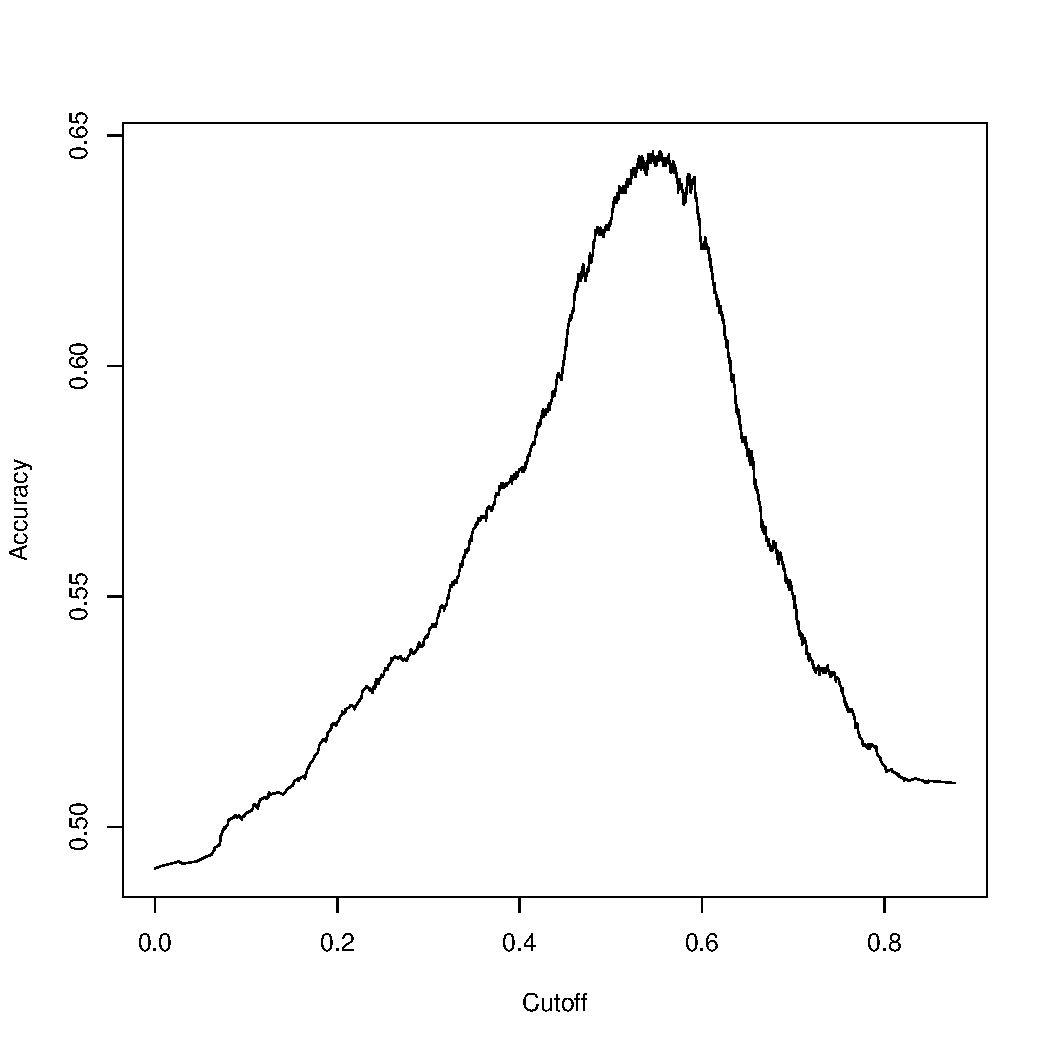
\includegraphics[width=0.9\textwidth]{t3/acc_scaled}
    \caption{Accuracy Curve on scaled dataset logistic regression model during last fold of ten-fold cross-validation}
    \label{fig:t3_acc_scaled}
\end{figure}

\begin{figure}[H]
  \centering
    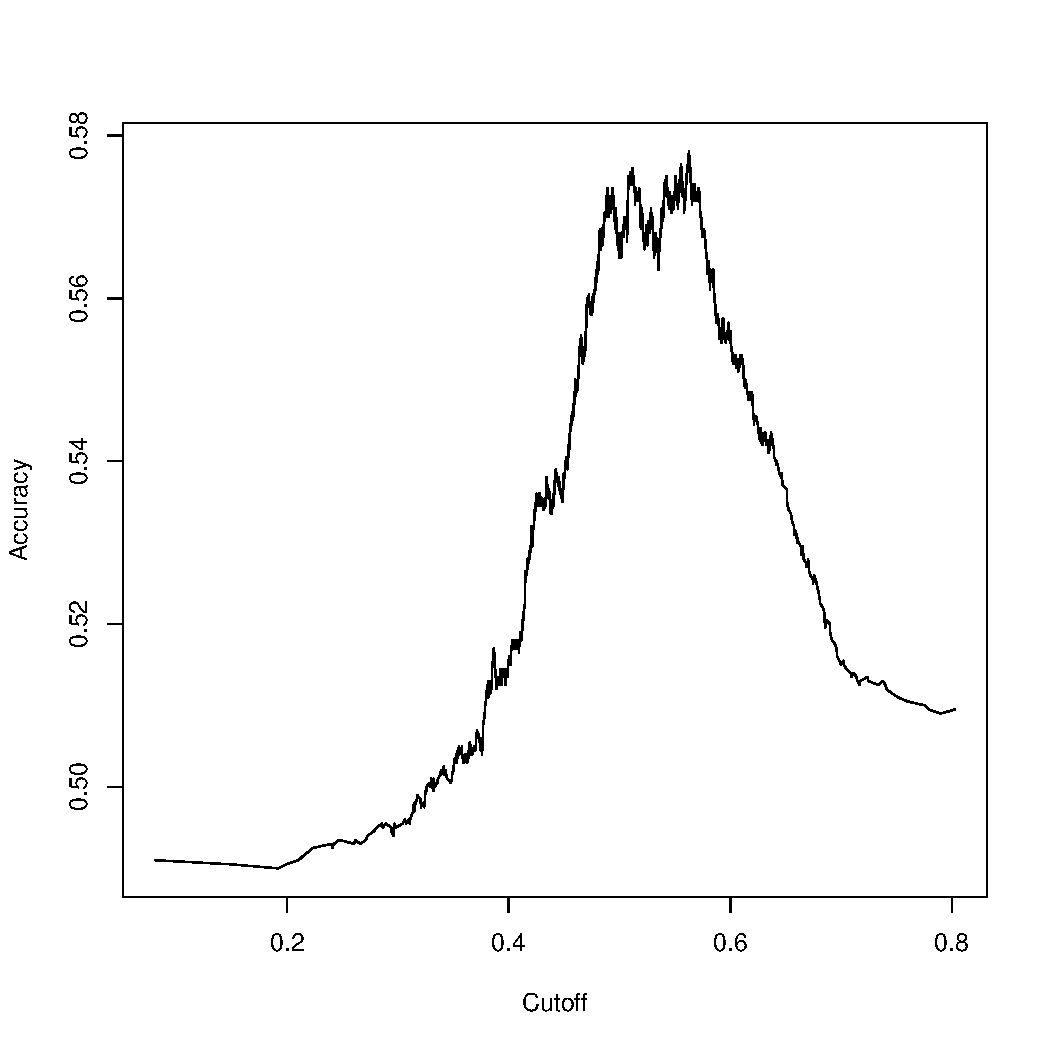
\includegraphics[width=0.9\textwidth]{t3/acc_low_reg_hl}
    \caption{Accuracy Curve on combination of low-level attributes and regressed high-level attributes logistic regression model during last fold of ten-fold cross-validation}
    \label{fig:t3_acc_low_reg_hl}
\end{figure}

\pagebreak\subsection{Predicting the unclassified dataset}
Prediction is made by using the best model built from the original dataset utilizing the 7 regressed high-level components and 21 low-level components inside ten-fold cross-validation. This model is saved at \textit{models/best\_nnet.rda} and loaded to perform classification on the unknown data. Since a result of 0.613 was formed using the evenly distributed train100k dataset during ten-fold cross-validation, one can expect a similar result in classifying the unknown dataset.

Using \textit{lm} gives the new seven high-level components for the new dataset and prediction is performed by applying the aforementioned model and results are saved to a CSV file.

\subsection{Conclusion}
Results show that combination of low-level attributes and regressed high-level attributes is slightly better than just low-level attributes. However, one should look into improving the calculation for the high-level components by refining the linear regression technique used. Feature interaction and better feature selection could provide help also.  
 
Using all the data is clearly useful but further understanding of the data is necessary to get better classification. It's clear that classification of \textit{H1} needs to be fine-tuned to reduce the overall average misclassification rate of high level attributes.

The problem is hard to classify due to small sample size and dataset imbalance. Advanced techniques may help such as distributed parallel techniques with a much larger dataset\cite{panda}.
\pagebreak
    \lstset{
	frame=single,
        breaklines=true,
	postbreak=\raisebox{0ex}[0ex][0ex]{\ensuremath{\color{red}\hookrightarrow\space}}
     }

\bibliographystyle{plain}
\bibliography{bibliography}

\end{document}
